% Chapter 2 of the Thesis Template File
%   which includes bibliographic references.

%Chapter 2: Related Work  
%1) Introduction paragraph summarizing the flow/content/structure of the Related Work, while describing how the areas of related work are logically connect to your work  
%2) Related area 1 
%3) Related area 2  
%4) Related area 3
%5) Within each related area, point out in what why your work is different from the existing work.

\chapter{Related Works}

\section{Introduction}
Software defined radios have been used in a number of applications, although most of these applications are with RF communications and not usually for remote sensing.  While as far as the author has determined, this is the first application of using an off the shelf software defined radio for a radiometer in remote sensing for soil moisture measurements, there has been similar applications done using software defined radios are equipment that is similar to a software defined radio.  This chapter will look at related works that involve applications in radio astronomy, related applications to RFI mitigation and radiometers that have similar hardware to our software defined radiometer.

\section{Radio Astronomy Examples}
Radiometers used in radio astronomy is nothing new and has been used for some time now[\cite{Ohm}]. There are similarities between radio astronomy and remote sensing of the ground.  Both are using a radiometer to listen to a source of interest.  With radio astronomy the basic principle is that a hot source such as a star will produce more noise than the cooler background of space.  In remote sensing we are looking at the overall change of the source to determine its characteristics.  Both cases are measuring the total power of the noise and based on that information we can determine some properties of the source we are looking at.
For our software defined radiometer however, we are looking at the ground and we are using the radiometer for soil moisture instead of measuring stars and other points of interest in the sky.  While the fundamentals is the same for either radiometer some adjustments need to be made because a radiometer that is looking at the sky often sees a cooler brightness temperature whereas a radiometer looking at the ground sees a much warmer brightness temperature.  This is due to the albedo of the Earth having a much warmer noise temperature then what you find with radio astronomy[\cite{Tiuri}].

\subsection{Shirleys Bay Radio Astronomy Consortium}
The Shirleys Bay Radio Astronomy Consortium (SBRAC) located in Smiths Falls, Ontario is using the USRP software defined radio in conjunction with GNURadio.  SBRAC has successfully used this configuration to obtain radio astronomy data by looking at the hydrogen line at 1420.4058 MHz [\cite{Leech2007}].  The person in charge of this facility, Marcus Leech, contributed software to the GNURadio specifically for radio astronomy applications.  It was this software branch that was used as the base for the GNURadio program that was used in this thesis.  Marcus Leech continue to contribute to the GNURadio community and continues to provide support for these functions as well[\cite{Leech}].

\subsection{Grand Valley State University}
Another example of a software defined radio used as a radiometer is from students at the University of Illinois and Grand Valley State University that built a software defined radio to listen to emissions from Jupiter[\cite{Behnke}].  This software defined radio was built using an Analog Devices AD9460 and a Xilinx Spartan-3E-500 FPGA to build the SDR itself.  A RF front end was also built to filter and amplify the signal coming into the SDR.  Finally, this group also used GNURadio to interface to and talk to the SDR and used both Python and wxGUI to build a working interface.  The students reported that the SDR radiometer worked well and was able to do so at a low price point.

\section{RFI Mitigation}
Radio Frequency Interference (RFI) is a common problem with a nearly all radiometers.  This problem is often exasperated with satellite radiometers since those radiometers see a large area on the ground.  Previous missions such as the Soil Moisture Ocean Salinity (SMOS) satellite has numerous issues with RFI that skews the data that they collect.  There have been a number of methods to either work around the RFI or attempt to filter it using mechanical filters.  University of Michigan has done a number of experiments in detection and mitigation of RFI with the use of mechanical filters [\cite{DeRooRFI}].  And a number of papers have been published on the detection of RFI in radiometers [\citep{DeRoo}][\cite{Forte}].

In all of these cases the radiometers used do not retain frequency information and thus must use other methods to detect and try to mitigate the signal.  In this thesis we cover a way to mitigate RFI and are able to do so using software to define a filter to notch out the offending signal.  Detection in a software defined radio radiometer is easier as we have both power and frequency information to design the filter.

\section{Other Digital Radiometers}
A digital radiometer is not a new concept.  Early radiometers often digitize the analog voltage information from the square-law detector and then send that information to a computer for storage or analysis[\cite{Ruf}].  

As a pre-cursor to a software defined radio, some radiometers also digitize the incoming RF signal, but under-sample this information.  Since only power is the only information desired for these radiometers, this was acceptable.  However, these radiometers did often use the same components you might find in a software defined radio such as an A/D converter and a FPGA for basic signal processing.  These components however were used in different ways.

\subsection{Direct Digital Sampled Radiometer}  
Iowa State University owns a 1.4 GHz, dual polarization, correlating radiometer that is in use by Dr. Brian Hornbuckle and his research team.  This radiometer was built at the University of Michigan and put into service at ISU in 2006.  The ISU radiometer is unique in that it is one of the few direct sampling radiometers in use\cite{Erbas}.  This radiometer takes the RF signal, amplifies and filters the signal, and then sends it directly to an analog to digital converter.  At the time the ISU radiometer was built an A/D that is able to sample accurately at 1.4 GHz was expensive and hard to come.  However, the ISU radiometer does not sample at 2.8 GHz or above, instead it samples at 1.4 GHz.  The ISU radiometer is able to do this because it is only interested in power information.  This means that we are not interested in recreating the entire signal and therefore we can under-sample the signal.  The A/D data is then sent to a Field Programmable Gate Array (FPGA) which then processes the data.  The ISU radiometer is also a correlating radiometer which means that it looks at both the vertical polarization (V-Pol) and the horizontal polarization (H-Pol) and then correlates this information[\cite{Fischman2001}]. 

One reason why these devices were used differently from a SDR was due to cost.  Most radiometer operations happen at 1.4 GHz or above.  A/D converters at these higher frequencies become more expensive and harder to obtain.  In recent years however, these costs have come down.

The major difference between other digital radiometers and what is discussed in this thesis is that we retain both phase and magnitude information and instead mimics a traditional radiometer in software by summing and squaring the I and Q values and then running this information through a low-pass IIR filter.  By retaining this information, we can perform a more in-dept analysis of the signal coming into the radiometer which allows for greater agility in the system.
%---------------------------------------------------------


%\subsection{RF Front End Design}

%The RF front end plays a critical role in a radiometer as the primary function is to amplify the signal so that it is easier to detect the changes in power or noise temperature.  This amplification comes with a cost that the LNA itself will contribute to the noise and this contribution is unwanted.  Therefore, we want to minimize the contribution and maximize the amplification of the noise we are looking at.  This Noise Figure (NF) is a metric we used to show how well a LNA amplifies a signal while keeping its contribution to the noise to a minimum.  Well engineered LNAs are now capable of producing very low noise figure numbers and are relatively inexpensive.  

%A typical design is a 3 stage system that uses 2 bandpass filters to help maintain the signal to the band of interest.  A traditional radiometer requires the use of bandpass filters since most LNAs have a fairly large operating bandwidth.  The filters ensure that the radiometer is operating in the band of interest, in our case the L-band from 1400 to 1426 MHz.  

%The software defined radio radiometer however does not require bandpass filters added.  There are two reasons for this.  One, the sampling rate set on the software defined radio sets a bandwidth and thus will limit the frequencies we are listening to.  Second, if needed additional filters can be created in software.  There is a cost to these filters in that additional processing power is needed, but otherwise they can be added with no additional cost to the system. 

%\subsection{Existing ISU RF Front End}

%The existing ISU radiometer RF Front end uses a series of cascading low noise amplifiers (LNAs) that increase the power from the antenna while contributing a minimum amount of noise to the system [\cite{Erbas}].  In addition, the current ISU RF front end uses bandpass filters to narrow the bandwidth to the desired 1400 to 1425 MHz that we wish to monitor.  While these are not needed with the addition of the software defined radio, since we can filter in software, they do not contribute much in terms of the noise temperature, and as passive components do not impact the performance of the radiometer as much as the LNAs do.

%{\begin{figure}[h!tb] 
%\centering
%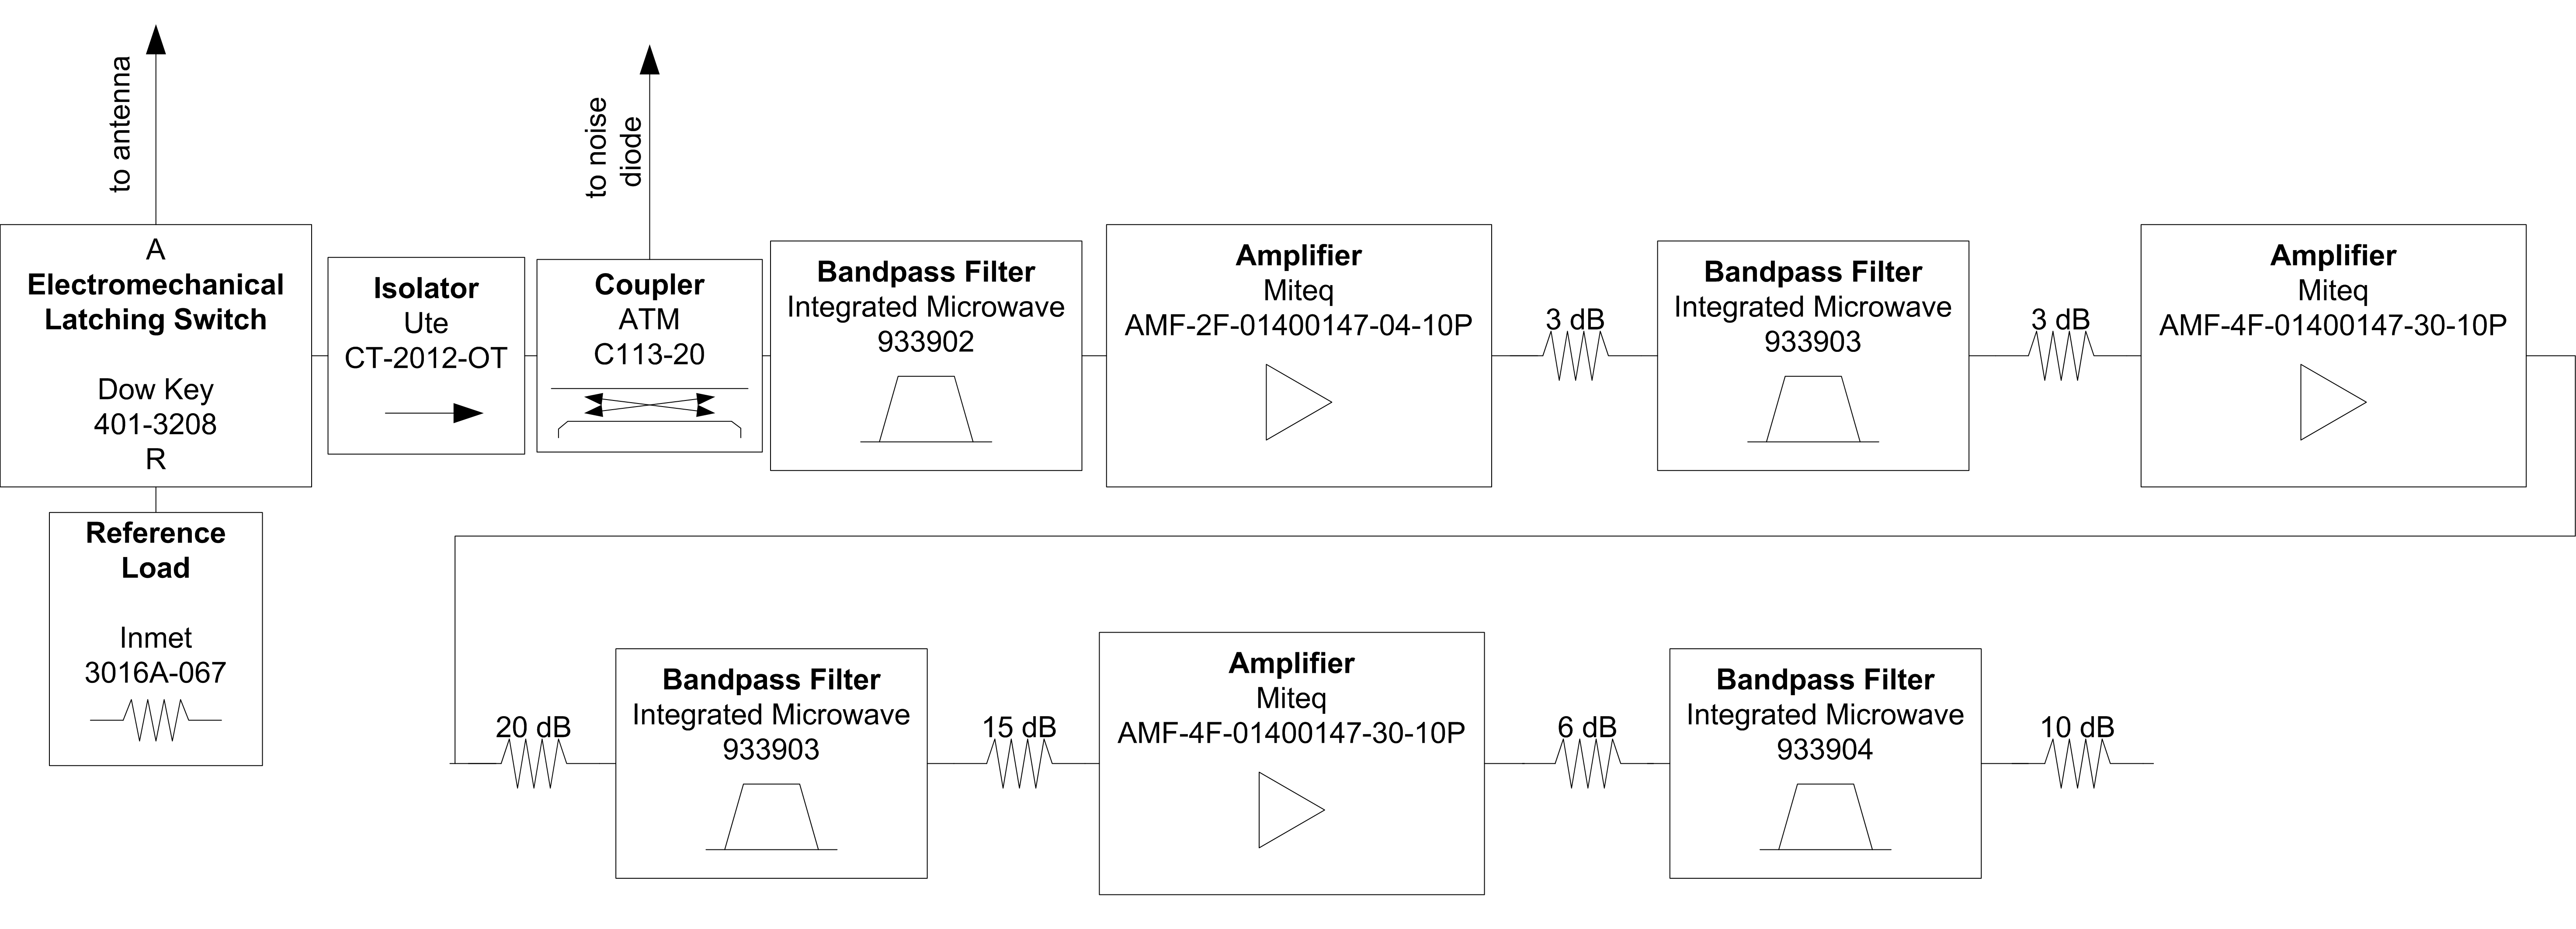
\includegraphics[width=17cm]{Images/ISU_rf_block.png}
%\isucaption{A block diagram provided by the University of Michigan that shows the components used in the ISU RF front end.}
%\label{ISU_rf_block}
%\end{figure}
%}

%As it can be seen in Figure \ref{ISU_rf_block} the current ISU rf front end uses a series of amplifiers, filters and attenuators to amplify and filter the incoming signals.  The attenuators are used to ensure that we do not overload the front end of the LNA proceeding it in the chain.  This RF chain provides us a spectrum from 1400 MHz to 1425 MHz and gives us a total gain of approximately 81 dBm.  This raises the noise floor to approximately -30 dBm which makes it very easy to detect with both a square-law detector and the software defined radio.  The performance of the ISU front end was confirmed by using a spectrum analyzer to look at the output signal and power output.  The spectrum analyzer output can be seen in Figure 

%{\begin{figure}[h!tb] 
%\centering
%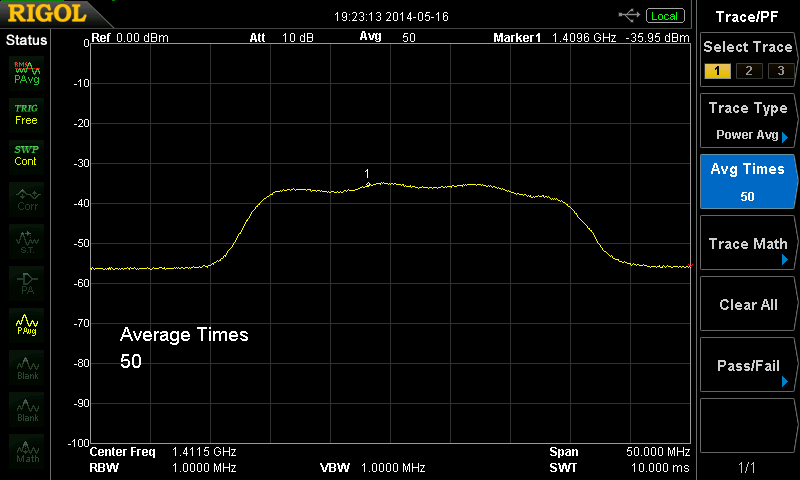
\includegraphics[width=17cm]{Images/radlidoff.png}
%\isucaption{A screenshot taken from a spectrum analyzer showing the filters and amplification done by the ISU Radio RF front end.}
%\label{ISU_rf_spectrum}
%\end{figure}
%}

%The ISU Radiometer front end was dismantled and was used for the experiments used in this thesis.  The LNAs and bandpass filters were kept intact to be used for experimentation.  While the bandpass filters were not needed for the software defined radio, since we were comparing our data to a square-law detector, they were still required for that device so that both the SDR and the Square-law detector could be looking at approximately the same signal.

%\subsubsection{A note about the ISU RF Front end}

%During the work on this thesis a few issues came up with the ISU RF front end that was used.  When work began on this thesis, it was assumed that the problems that were found with this hardware was limited to the digital portion of the radiometer.  This meant that the RF front end was performing as expected.  At first, early tests on the ISU RF front end seemed to confirm this as the output seen on a spectrum analyzer appeared to be normal.  However, further testing started to show unusual behavior.  Later, it was discovered that the ISU RF front end was prone to malfunctioning under certain conditions.  These conditions seemed to occur when the RF front end was moving on it's platform and even the lid to the box containing the RF front end would affect it.  

%A test was done to show this effect with the lid, and further information about the rotation affect is discussed in Appendix 2 in regards to the E E 518 laboratory experiment. For the lid experiment, a spectrum analyzer was hooked up to the ISU RF front end.  With the lid off, you can see what appears to be a normal signal that we would expect from the radiometer in Figure \ref{ISU_rf_spectrum}.  However, in Figure we placed the lid on the radiometer and the results are quite different.  Changes to the signal were observed in real time as the lid was placed on the radiometer and it was clear that this was also causing the radiometer to produce undesirable results.  

%{\begin{figure}[h!tb] 
%\centering
%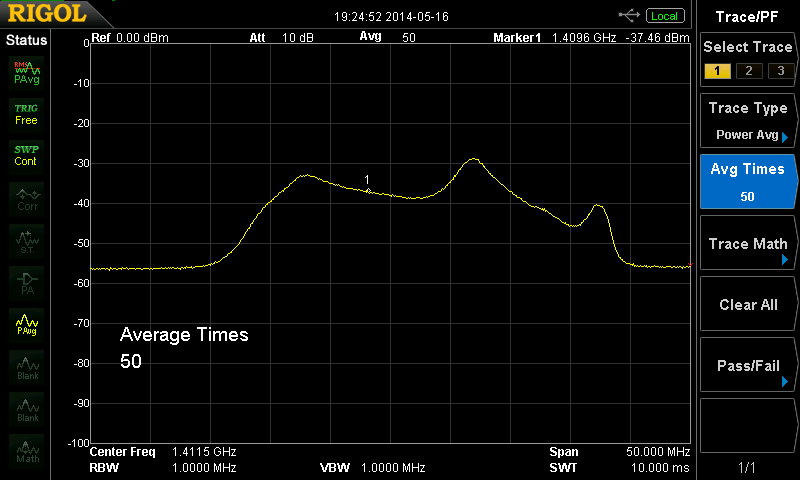
\includegraphics[width=17cm]{Images/lidpart.png}
%\isucaption{A screenshot taken from a spectrum analyzer showing the affect of the radiometers lid as it was placed on the radiometer.}
%\label{lid_on}
%\end{figure}
%}

%It was clear that there is something happening with the ISU RF front end.  This also points out another use for the addition of the software defined radio.  The old ISU radiometer system under-sampled the signal and so frequency information was lost.  Without hooking up something like a spectrum analyzer there would be no way for any to know what was happening with the ISU radiometer.  However, with the SDR we now have power and spectrum information.  In fact, it was during the E E 518 laboratory that we noticed a problem with the ISU radiometer and we discovered this by looking at the data that was captured by the SDR.  It was due to these issues that came up that the RF front end was rebuilt. 

%Work was done to re-stabilize and make the ISU radiometer front usable for the experiments used in this thesis.  First, all non-essential equipment was deactivated and powered down.  This included the on board microcontroler, the A/D converters and the FPGA unit that was originally used in this radiometer.  The thermal electric coolers were also deactivated as well.  Since the LNAs were in a temperature controlled room, they were not needed for these experiments.  

%Next, the LNAs were powered from a lab bench power supply instead of the power supplies that were used in the radiometer.  It is theorized that the power supplies feeding the radiometer may have been damaged due to water that had entered the case and were no longer stable in the power they provided.  To eliminate any issues, they were removed and a new and known to be working lab power supply was used to power both the LNAs and the square-law detector circuitry.   

\section{Software Defined Radio Theory of Operation}


\subsection{Software Defined Power Detection}

A traditional radiometer uses a square-law detector which takes the input signal and produces a voltage that is proportional to the square of the voltage.  This allows us to take an analog RF signal and convert the noise voltage that for all intense and purposes has a mean value of zero, and produce a noise power.

For a SDR, the incoming signal is sampled and converted to I/Q values by the hardware within the SDR.  The I/Q values together can be used to recontruct both the phase, frequency and amplitude information of the signal and can do so much more accurately then if we just recorded the frequency and amplitude information.  In GNURadio we are then able to square these values within software which give us our peak voltage of the signal.  This block in GNURadio mathematically performs what is shown in equation \ref{sdr_x2}.

\begin{equation}\label{sdr_x2}
I^2+Q^2 = P_{out}
\end{equation}

Therefore, like the analog square-law detector we are taking peak voltage values, which has an equivalent noise voltage and a mean value of zero, and square them to produce a noise power that is proportional to the square of this amplitude.

Like the analog square-law detector, this signal will fluctuate rapidly and to improve the sensitivity of the radiometer we wish to integrate this signal.  We now want to look at how we can replicate a RC filter or integrator in the software defined radio.

\subsection{Software Defined Integrator}
A RC filter is analogous to an integrator where the R and C values determine our time constant and our integration time for the filter[\cite{Aitken}].  We know a RC filter is analogous to an integrator by looking at equation \ref{eq:rc_int}.  A SDR however operates in the digital domain at discrete intervals.  One type of filter that can be used is the Infinite Impulse Response (IIR) filter. 

\begin{equation}\label{eq:rc_int}
\frac{1}{RC}\int{V_idt}
\end{equation}


To begin with, we look at what an analog RC filter looks like. 

{\begin{figure}[h!tb] 
\centering
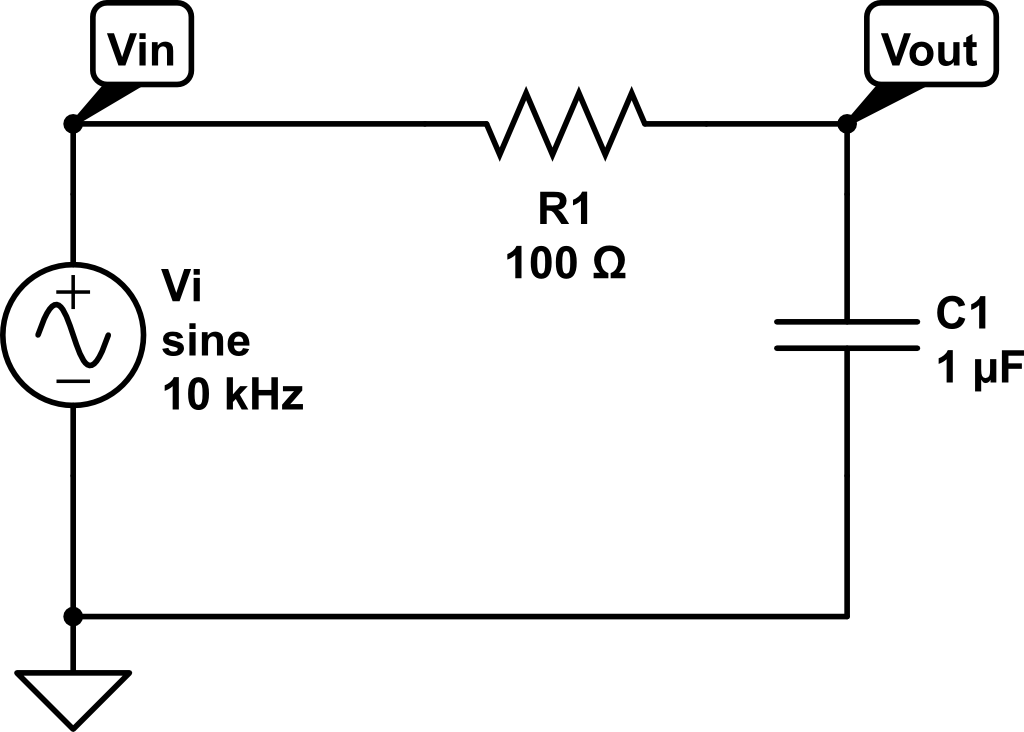
\includegraphics[width=10cm]{Images/rc-circuit.png}
\isucaption{A simple RC circuit}
\label{rc_circuit}
\end{figure}
}

This circuit can be represented by equation \ref{eq:rc_circuit_eq}.

\begin{equation}\label{eq:rc_circuit_eq}
\frac{V_{in}-V_{out}}{R}=C\frac{dV_{out}}{dt}
\end{equation}

A Finite Impulse Response (FIR) filter is a digital filter that can take an impulse signal and decays to zero after a finite number of iterations.  This type of digital filter can be represented by equation \ref{FIR_Eq} which mathematically expresses the FIR Filter.

\begin{equation}\label{FIR_Eq}
y_n=\displaystyle\sum\limits_{i=o}^{P-1} c_ix_{n-i}
\end{equation}

This simply says that the nth output is a weighted average of the most recent P inputs.  

An Infinite Impulse Response (IIR) filter is the same as the FIR filter, except that we add a summation term which feeds back the previous output.

\begin{equation}\label{IIR_eq}
y_n=\displaystyle\sum\limits_{i=o}^{P-1} c_ix_{n-i}+\displaystyle\sum\limits_{j=1}^{Q} d_jy_{n-j}
\end{equation}

Equation \ref{IIR_eq} shows that a FIR filter is a IIR filter, except that $Q=0$[\cite{Cross}].  

To get a better understanding on how the digital IIR filter relates to the RC filter analog, we can look at the Fourier Transform and the relationship of the input to the output in the frequency domain.

\begin{equation}\label{Fourier_IIR}
H(f)=\frac{\displaystyle\sum\limits_{j=o}^{P-1} c_je^{-2\pi ijfT}}{1-\displaystyle\sum\limits_{k=1}^{Q} d_ke^{-2\pi ikfT}}
\end{equation}

In equation \ref{Fourier_IIR}, $f$ is our frequency in Hz and $T$ is the time between samples in seconds and is related to our sampling frequency.

We now want to show the link between our analog RC circuit and the IIR filter.  Looking at equation \ref{eq:rc_circuit_eq}, which represents the differential equation relating the input voltage $V_{in}$ to the output voltage $V_{out}$, we can substitute for input and output of our IIR filter.  Since we are now in the time domain, we need to define what $T$ is and we can do that using equation \ref{sampling_rate_eq}.

\begin{equation}\label{sampling_rate_eq}
T=time between samples=\frac{1}{sampling rate}
\end{equation}

We can now relate our input voltage to the input to our IIR filter and the output voltage to the output of our IIR filter.

\begin{equation}\label{input_IIR}
x_n=v_{in}(nT)
\end{equation}

\begin{equation}\label{output_IIR}
y_n=v_{out}(nT)
\end{equation}

We can now rewrite our difference equation with $x_n$ and $y_n$.

\begin{equation}\label{diff_xn_yn}
\frac{x_n-y_n}{R}=C\frac{y_n-y_{n-1}}{T}
\end{equation}

Finally, we can solve for $y_n$ which results in our final equation for showing how a IIR filter is related to an RC filter.

\begin{equation}\label{final_IIR_RC}
y_n=\frac{T}{T+RC}x_n+\frac{RC}{T+RC}y_{n-1}
\end{equation}

It can be seen that an IIR filter can have the same frequency response as we expect from an analog RC filter.  As our sampling rate approaches infinity, the approximation gets closer to the original response from the analog RC circuit.  

For the cutoff frequency of a RC circuit, we know that it has the relationship shown in equation \ref{RC_relationship}.

\begin{equation}\label{RC_relationship}
f_c=\frac{\sqrt{3}}{2\pi RC}\rightarrow RC=\frac{\sqrt{3}}{2\pi f_c}
\end{equation}

The $RC$ term gives us our time constant of the circuit and can be used to calculate out our coefficients.  We are not concerned about the actual values of R and C with our IIR filter, instead we just need the product of R and C.  

In GNURadio most of the work is done for us.  We can simply enter in our desired cutoff frequency and GNURadio will calculate our IIR filter coefficients.  However, this shows that an IIR filter works much like an analog RC low pass filter.

Like a traditional radiometer, the SDR will use an antenna to look at the target of interest.  SDRs still use a RF stage that takes the power from the source and amplifies it.  The difference though begins after that.  A SDR will then sample and generate I and Q values that represents the amplitude and phase of the signal.  From there, this data is sent to a computer to be processed.  We can then use this information to calculate the power that is being seen.  In addition, we can manipulate the signal in other ways such as applying a filter to filter out an unwanted source.

\subsection{SDR Radiometer Summary}

As we have shown the two of the major components of a traditional radiometer, the power detection and integration of the signal can be replicated in software and therefore can be implemented in a software defined radio.  The information can now be stored, displayed or both for further analysis.  

There is one component of the software defined radio that we are not able to implement in software and that is with the signal amplification.  This however does play a major role in the performance of the radiometer and is a key element that should not be overlooked.  While this is not implemented in software, it still plays a critical role in our software defined radio radiometer. 

\subsection{RF Front End}

Hardware with a software defined radio still plays a critical role.  A traditional software defined radio will focus on digitizing the signal as soon as possible and the hardware used will be focused on performing that critical digitizing process.  For a software defined radio radiometer, we still want to digitize as soon as possible, but we also need to consider our noise factor.  Most software defined radios are designed for communication purposes such as implementing 802.11b or other wireless protocols.  In these scenarios a higher noise factor is not as detrimental to the overall system as it is with a radiometer.  This is because we have a known signal that is magnitudes greater than the noise floor.  In a radiometer however, we do not have this large separation between the information we need and the noise of the system.  And so our noise factor is a more critical component.  

To counter this, we use Low Noise Amplifiers to amplify the signal but it can also help lower our noise factor.  The first LNA in the chain contributes a large amount to our noise factor, so by selecting a LNA that has a low noise factor, it reduces the noise factor for the system.  This can be shown by looking at the equation that calculates our noise factor.

\begin{equation}\label{noise_factor}
F=F_1+\frac{F_2-1}{G_1}+\frac{F_3-1}{G_1 G_2}+\frac{F_4-1}{G_1 G_2 G_3}+\cdots +\frac{F_n-1}{G_1 G_2 G_3 \cdots G_{n-1}}
\end{equation}

While additional components do add to the noise figure, their contribution is significantly lower than the first LNA put in the RF chain.

This however is the only major change we need to do for doing radiometer work with an off the shelf radiometer.  The rest will be done within software which is the principal reason for using a software defined radio.

\section{General Specifications}
In general, since we are digitizing the signal early in the RF signal chain, the noise figure of the RF components in the SDR do not add a significant amount of noise to the system.  Additional performance metrics that require examination include how much bandwidth the system can handle.   The information below outlines the specification of the devices used and its impact on the performance of the SDR as a digital radiometer.   

\section{Comparison of a Software Defined Radio Radiometer vs Traditional Radiometer}

As outlined above, a software defined radio implements a traditional radiometer but in the digital domain.  For power detection, we simply sum the squares of the I and Q values that have been sampled by the software defined radios analog to digital converters.  As with a traditional radiometer, we also want to filter this information to remove much of the jitters that comes from the rapid fluctuations in the power readings.  This is done using an IIR low pass filter, which mimics a traditional RC low pass filter.  Once completed, we now have the total power reading from the radiometer and we can now store, display or do both with this information.  

A traditional radiometer may also use an analog to digital converter in order to digitize the analog voltage from the square-law detector.  Because the sample rate of this voltage is low, almost any analog to digital can be used for this.  At this point however, there is no frequency information, only the magnitude information is being retained and recorded.

